%% ****** Start of file apstemplate.tex ****** %
%%
%%
%%   This file is part of the APS files in the REVTeX 4 distribution.
%%   Version 4.1r of REVTeX, August 2010
%%
%%
%%   Copyright (c) 2001, 2009, 2010 The American Physical Society.
%%
%%   See the REVTeX 4 README file for restrictions and more information.
%%
%
% This is a template for producing manuscripts for use with REVTEX 4.0
% Copy this file to another name and then work on that file.
% That way, you always have this original template file to use.
%
% Group addresses by affiliation; use superscriptaddress for long
% author lists, or if there are many overlapping affiliations.
% For Phys. Rev. appearance, change preprint to twocolumn.
% Choose pra, prb, prc, prd, pre, prl, prstab, prstper, or rmp for journal
%  Add 'draft' option to mark overfull boxes with black boxes
%  Add 'showpacs' option to make PACS codes appear
%  Add 'showkeys' option to make keywords appear
\documentclass[aps,prl,twocolumn,groupedaddress]{revtex4-1}
%\documentclass[aps,prl,preprint,superscriptaddress]{revtex4-1}
%\documentclass[aps,prl,reprint,groupedaddress]{revtex4-1}

% You should use BibTeX and apsrev.bst for references
% Choosing a journal automatically selects the correct APS
% BibTeX style file (bst file), so only uncomment the line
% below if necessary.
%\bibliographystyle{apsrev4-1}
\usepackage{amsmath}
\usepackage{amsfonts}
\usepackage{amssymb}
\usepackage{graphicx}
\usepackage{tabularx}
\usepackage{booktabs}
\newcolumntype{Y}{>{\centering\arraybackslash}X}

\begin{document}

% Use the \preprint command to place your local institutional report
% number in the upper righthand corner of the title page in preprint mode.
% Multiple \preprint commands are allowed.
% Use the 'preprintnumbers' class option to override journal defaults
% to display numbers if necessary
%\preprint{}

%Title of paper
\title{Beyond Boost-invariant Initial Condition for Relativistic Heavy Ion Collision Simulation}

% repeat the \author .. \affiliation  etc. as needed
% \email, \thanks, \homepage, \altaffiliation all apply to the current
% author. Explanatory text should go in the []'s, actual e-mail
% address or url should go in the {}'s for \email and \homepage.
% Please use the appropriate macro foreach each type of information

% \affiliation command applies to all authors since the last
% \affiliation command. The \affiliation command should follow the
% other information
% \affiliation can be followed by \email, \homepage, \thanks as well.
\author{Weiyao Ke}
%\email[]{Your e-mail address}
%\homepage[]{Your web page}
%\thanks{}
%\altaffiliation{}
\affiliation{Duke University}

%Collaboration name if desired (requires use of superscriptaddress
%option in \documentclass). \noaffiliation is required (may also be
%used with the \author command).
%\collaboration can be followed by \email, \homepage, \thanks as well.
%\collaboration{}
%\noaffiliation

\date{\today}

\begin{abstract}
Abstract:
\end{abstract}

% insert suggested PACS numbers in braces on next line
\pacs{}
% insert suggested keywords - APS authors don't need to do this
%\keywords{}

%\maketitle must follow title, authors, abstract, \pacs, and \keywords
\maketitle

% body of paper here - Use proper section commands
% References should be done using the \cite, \ref, and \label commands
\section{Introduction}
	Ultra-relativistic heavy ion collision produces the hottest medium in the lab since the first operation of RHIC at Brookhaven National Lab. 
	The transient hot and dense state of matter with a life time of femtoseconds is known as quark-gluon plasma (QGP). 
	Viscous hydrodynamics modelling with thermalization at early stages very well describes the experimental data. 
	An unexpectedly low shear viscosity to entropy ratio $\eta/s$, close to the quantum lower bound from AdS/CFT correspondence, is needed to explain the observed momentum anisotropy.
	The system therefore behaves like an almost perfect liquid, revealing the strongly coupled nature of the problem.
	This motivates large effort to quantify the transport properties of this new state of matter.
	
	Modelling is essential to the problem. 
	Since quarks and gluons always hadronize and what can be detected directly are hadrons and decay products, it requires modelling time evolution of both QGP and hadron final states in order to compare with experimental data. 
	Also, due to the lack of knowledge of initial stages of the collision such as nuclear wave function and how the system undergoes fast thermalization and isotropization, models of initial condition are indispensable.
	
\section{``Standard Model" of Soft Physics}
	The present "Standard Model" of soft sector in relativistic heavy ion collision consists of four stages.
	\begin{itemize}
		\item Fast thermalization. 
		Immediately after the collding of two nuclei, the fireball is far from thermal equilibrium. However, in less than $1 \textrm{ fm/c}$, the system is already close to local thermal equilibrium. 
		The reason of this fast thermalization is still not clear.
		\item Hydrodynamical expansion of QGP. 
		Relativistic viscous hydrodynamics describes the expansion of QGP by solving energy-momentum and charge conservation,
		\begin{eqnarray}
			\partial_\nu T^{\mu\nu} &=& 0, \\
			\partial_\nu N^{\nu} &=& 0. 
		\end{eqnarray}
		Hydrodynamics translates initial spatial anisotropy into momentum space anisotropy reproducing the famous harmonic flows. 
		Equation of state of hot QCD matter is an input as calculated from Lattice QCD.
		3+1 d hydrodynamics \cite{Iurii:2014vhlle}

		\item Statistical hadronization, freezeout. 
		As temperature drops and hydrodynamics does not apply, the system is particularized by statistical sampling hadrons from particle distribution function, the Cooper-Frye formula,
		\begin{eqnarray}
			E\frac{\mathrm{d}N_i}{\mathrm{d}^3p} = \int_\Sigma f_i(x, p)p^\mu,\mathrm{d}^3\sigma_\mu.
		\end{eqnarray}
		\item Final state scattering. 
		The system after freezeout is still dense enough to allow hadronic scattering. 
		Transport model such as UrQMD is utilized to solve the Boltzmann equation,
		\begin{eqnarray}
			\frac{\mathrm{d}f_i(x, p)}{\mathrm{d}t} = C_i(x, p).
		\end{eqnarray}
	\end{itemize}


\section{Large/Small system collision and Boost-invariance Approximation}
	The matter produced in heavy ion collision expand rapidity in the beam direction. So it is convenient to express the system in terms of curvilinear coordinates $(\tau, x, y, \eta_s)$. 
	With $x, y$ remains the same as Cartesian coordinates transverse to beam direction, $\tau$ and $\eta_s$ are known as local time and space-time rapidity of the system,
	\begin{eqnarray}
		\tau = \sqrt{t^2 - z^2} &,& \eta_s = \frac{1}{2}\ln\left(\frac{t+z}{t-z}\right) \\
		t = \tau \cosh \eta_s &,& z = \tau \sinh \eta_s.
	\end{eqnarray}
	These coordinates transforms under lorentz boost along $z$ direction as,
	\begin{eqnarray}
		(\tau, {\bf x_{\perp}}, \eta_s) \xrightarrow{L} (\tau, {\bf x_{\perp}}, \eta_s + \Delta)
	\end{eqnarray}
	
	A boost invariant solution of hydrodynamics is a solution without $eta_s$ dependence, therefore the solution looks the same in every frame related by a boost along beam axis. 
	For example, when nuclei are modelled by infinitely large uniform slab in transverse direction, the boost invariant solution in curvilinear frame $\tau s = const.$ recast into Cartesian coordinates,
	\begin{eqnarray}
		s = \frac{const.}{\sqrt{t^2 - z^2}}.
	\end{eqnarray}
	
	\section{TRENTo Initial Condition}
	Under the boost-invariant approximation, it is sufficient to specify the initial condition at mid-rapidity ($\eta_s = 0$). Various models were proposed to describe the entropy/energy deposition at mid-rapidity. 
	However, these models can be phenomenologically described with an effective model TRENTo \cite{Moreland:2014oya}. 
	TRENTo IC consist of three levels of parametrization,
	\begin{itemize}
		\item Binary nucleon-nucleon collision.
		\item Nuclear-nuclear collision.
		\item Mid-rapidity entropy deposition ansatz.
	\end{itemize}
	The first two steps are similar to the procedures of Monte-Carlo Glauber Model; however, TRENTo employs a much generalized entropy deposition formula.
	\subsection{Parametrization of Binarg Nucleon-nucleon collision}
	Impact parameter differential inelastic cross-section is parametrized in the eikonal limit,
	\begin{eqnarray}\label{dsigma_db}
		\frac{\mathrm{d}\sigma_{nn}}{2\pi b \mathrm{db}} = 1 - \exp\left(-\alpha T_{pp} (b)\right).
	\end{eqnarray}
	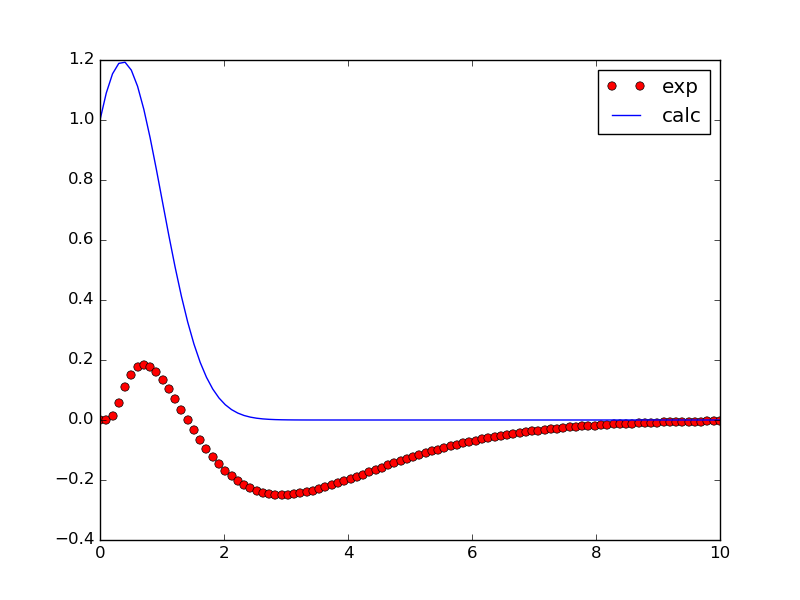
\includegraphics[width=\columnwidth]{pics/place_holder.png}
	$T_{pp}$ is the overlapping of nucleons' transverse density function $\rho(x_\perp)$, which is generally assumed to be normalized Gaussian,
	\begin{eqnarray}
		\rho(x_\perp) &=& \frac{1}{\sqrt{2\pi w^2}}\exp\left(-\frac{{x_\perp}^2}{2w^2}\right), \\
		T_{pp}(b) &=& \int \mathrm{d}{x}^2 \rho(x+\frac{b}{2})\rho(x-\frac{b}{2})
	\end{eqnarray}
	All the information of subnucleonic degrees of freedom is encoded in the coefficient $\alpha$, which is tuned to reproduce the inelastic proton-proton inelastic cross-section at a given energy,
	\begin{eqnarray}
		\int \mathrm{d}\sigma_{nn}(\alpha) = \sigma_{pp, inel}(\sqrt{s}).
	\end{eqnarray}
	Eq. (\ref{dsigma_db}) is then interpreted as the probability for two nucleon to collide with separation of $b$ and is realized via a Monte Carlo approach.
	\subsection{Parametrization of Nuclear-nuclear Collision}
	The penetrating of nuclei of ultra-relativistic collision takes much shorter time than the time scale of nucleon motion inside a nuclei; therefore, nucleon position fluctuation need to be taken into account. 
	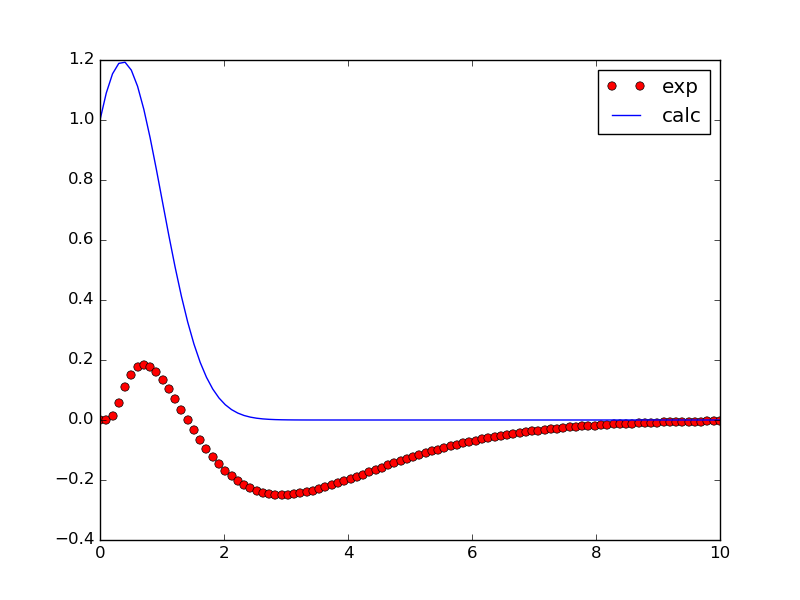
\includegraphics[width=\columnwidth]{pics/place_holder.png}
	In TRENTo, nucleons are sampled from a (deformed) Woods-Saxon density distribution and then projected onto the transverse plain. 
	Each pair of nucleons with one from projectile and the other from target nuclei is examined with the binary collision criterion. 
	Nucleons subject to at least one collision are called participants, and the rest, spectators.
	The contribution of participants from nuclei $\{A,B\}$ defines the nuclear thickness function:
	\begin{eqnarray}
		T_{A,B}(x_\perp) &=& \sum_{i \in Part A,B} \gamma_i. \rho(x_\perp- x_i), \\
		\gamma_i &\sim& \Gamma(k, k).
	\end{eqnarray}
	Note that the contribution from each participant nucleon is multiplied by a random variable $\gamma_i$ subject to $\Gamma$ distribution with unity mean and variance $1/k$. 
	This additional source of fluctuation is added to reproduce the negative binomial distribution of number of charged particle in minimum biased $pp$ collisions.
	\subsection{Entropy Deposition Ansatz}
	TRENTo assumes in the eikonal limit, immediately after the penetrating of the nuclei, entropy deposition are local function of nuclear thickness functions $T_{A,B}$. 
	Generalized mean ansatz provide a flexible way to parametrize this mapping,
	\begin{eqnarray}
	\left.\frac{\mathrm{d^3}s}{\mathrm{d}\eta_s \mathrm{d}x_\perp^2}\right\vert_{\eta_s = 0} &=& 	T_R\left(T_A, T_B; p\right),	\\
	T_R(x, y; p) &=& \left(\frac{x^p+y^p}{2}\right)^{\frac{1}{p}}.
	\end{eqnarray}
	With parameter $p$ various, this ansatz mimic a variety of initial condition models.
	\begin{center}
	\begin{tabularx}{0.45\textwidth}{c>{\centering\arraybackslash}m{2.0cm}>{\centering\arraybackslash}m{2cm} cX}
	\toprule[1pt]
	$p$	&	$-0.5$	 	&	$0.0$ 		& 	$1.0$		\\
	\midrule[0.5pt]	
	$\sim$ &		KLN		& 	EKRT		& 		Wounded Nucleon \\
	\bottomrule[1pt]
	\end{tabularx}
	\end{center}
	The ``$\sim$" sign in the table reminds that $T_R$ resembles the entropy deposition of different models for reasonable value of thickness function. 
	This parametrization allows interpolation between different initial condition models and is suitable for a model selection procedure to learn what is the most probable initial condition to explain the observed experimental data at mid-rapidity.
	A model to data comparison by Bayesian analysis has very well constrained $p$ to be close to zero.
\section{Rapidity Dependent Extension of TRENTo}
	Although many models are proposed to describe mid-rapidity initial condition, it is not very clear how to include rapidity dependent effect. In the same spirit of TRENTo, we tried to parametrize the rapidity dependent initial condition in a flexible and simple way, so that a model select procedure can be applied.
	
	Because of the success of TRENTo at mid-rapidity, the 3d-extension will preserve prediction of TRENTo at $\eta_s = 0$ and the entropy distribution immediately after the collision will be local function of $T_A$ and $T_B$,
	\begin{eqnarray}
	T_A(x_\perp), T_B(x_\perp) \rightarrow \frac{\mathrm{d^3}s}{\mathrm{d}x_{\perp}^2 \mathrm{d}\eta_s}\left(x_\perp, \eta_s\right)
	\end{eqnarray}
	Also for simplicity, it is assumed the rapidity dependece factorize from the transverse distribution $T_R$,
	\begin{eqnarray}
		\frac{\mathrm{d}S}{\mathrm{d}x_{\perp}^2 \mathrm{d}\eta_s}  &\propto& T_R(x_\perp) \frac{F(x_\perp,y)}{F(x_\perp,0)}\frac{\mathrm{d}y}{\mathrm{d}\eta_s}
	\end{eqnarray}
	
	Instead assuming any explicit form of the space-time rapidity dependence $F(x_\perp, \eta)$, we first parametrize its cumulants, and then reconstruct it (as function of rapidity) by inverse Fourier transform of its cumulant generating function,
	\begin{eqnarray}
	 	F(x_\perp,y) &=& \mathcal{F}^{-1}\{\tilde{F}(k)\} \\
	 	\ln \tilde{F} &=&  i \mu k - \frac{1}{2}\sigma^2 k^2 + i 	\gamma k^3  - \kappa k^4
	\end{eqnarray}
The	with the relation between particle's rapidity and space-time rapidity,
	\begin{eqnarray}
		\eta_s &=& \sinh^{-1}(\sqrt{K}\sinh(y)), K>1. 
	\end{eqnarray}
is used to obtain the final space-time distribution.

	Different rapidity dependent IC models can be mapped to different parametrization of cumulants. Two existing approach with the name "Shifted" or "Tilted" are listed in the first two rows.
	\begin{widetext}
	\begin{center}
	\begin{tabularx}{0.8\textwidth}{c *{4}{Y}}
	\toprule[1pt]
	Cumulants & mean &	std	& skewness	& kurtosis \\
	\cmidrule[0.5pt]{2-5}
		&	$\mu(x_\perp)$ & $\sigma(x_\perp)$& $\gamma(x_\perp)$  & $\kappa(x_\perp)$	\\
	\midrule[0.5pt]
	shifted & $\frac{1}{2}\ln\frac{T_A}{T_B}$ & const. &  $0$	&const.\\
	tilted & $0$ & const.& $T_A - T_B, \frac{T_A-T_B}{T_A+T_B}$	& const.\\
	general & $\frac{a}{2}\ln\frac{T_A}{T_B}$& b  & $c(T_A - T_B)$ & d \\
	\bottomrule[1pt]
	\end{tabularx}
	\end{center}
	\end{widetext}
	A shifted initial condition assumes that in asymmetrical collisions, particle production (local in transverse plabe) as function of rapidity resembles a Gaussian as symmetrical case, with its mean shifted to the center of mass rapidity $\frac{1}{2}\ln(T_A/T_B)$. A tilted initial condition modified the symmetrical distribution by a linear tilting,
	\begin{eqnarray}
	f_{asy}(\eta_s) = f_{sym}(\eta_s) (1+\alpha \eta_s)
	\end{eqnarray}
	with $\alpha$ a measure of the degree of asymmetry. 
	Two possible construction of degree of asymmetry are shown in the second row. 
	This first one is a dimensionfull quantity while the second is a dimensionless construction. 
	In the last row, we show a general case with the mean of the function proportional to the center-of-mass rapidity and the skewness proportional to the degree of asymmetry. 
	By varying the coefficients $a, c$, we are able to interpolate between this two types of assumption.
	
	\begin{figure}\label{regulation}
	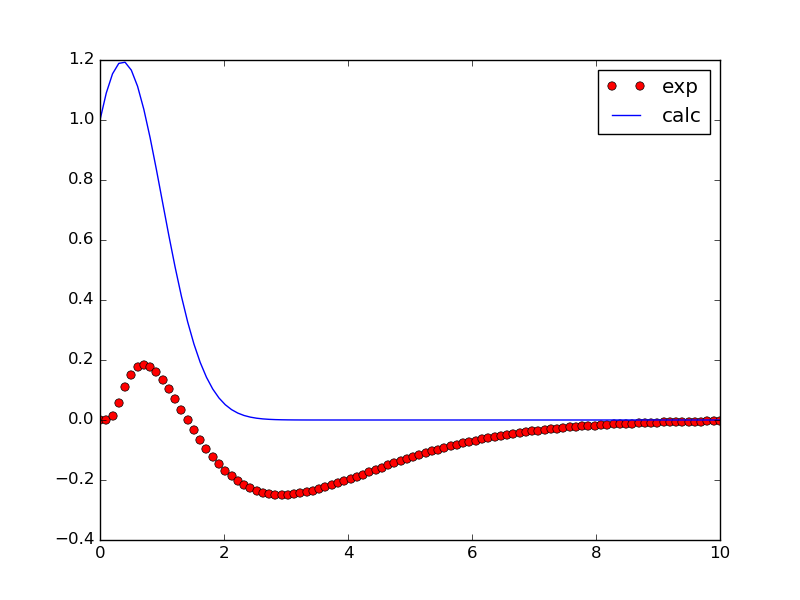
\includegraphics[width=\columnwidth]{pics/place_holder.png}
	\end{figure}
 
	However, the reconstructed function may not be well-behaved for relatively large degree of asymmetry. 
	From the left panel of Fig. (\ref{regulation}), with the increase of skewness, there is not a monotonic trend of change; also, the function goes to negative for large $|\eta_s|$
	This shows the importance of including higher order cumulants to regularize the behaviour of the generating function. 
	The conditions to ensure a positive definite Fourier transform are quite involved, but with the following substitution,
	\begin{eqnarray}
		\{\gamma, \kappa\} \rightarrow \{\gamma, \kappa\} \exp\left(-\frac{1}{2}\sigma^2k^2\right),
	\end{eqnarray}
	The negative region is suppressed and there is clear monotonic trend with the increase of skewness (right panel of Fig. (\ref{regulation}), the range of skewness showed in the plot covers the largest reasonable value in the initial condition. )
		
	Note that this substitution leaves the skewness and kurtosis intact, while contribution from higher order cumulants are included systematically.
	The distribution reconstructed with regularization produce and is positive and well behaved over a wide range of rapidity and skewness.

\section{Model to Data Comparison}
	The ultimate goal is to confront the calculations of hybrid model with different initial conditions to the experimental measurements, which will improve out knowledge of initial condition and expand model capability to look for rapidity related observables.
	Here the procedure of a model to data comparison with Bayesian analysis summarized. 
	\subsection{Parameter design}
	Hybrid model for heavy ion physics usually contains multiple parameters. 
	A 3d extension of the existing initial conditon introduce $4\sim5$ more parameters. 
	This constitutes a high dimensional parameter space $(p_1, p_2, ..., p_n)$, which makes it impractical to uniformly search the space. 
	A Latin Hypercube experimental design to sample parameters is preferable. 
	In such experimental design, parameters (properly normalized to live in $[0,1)^n$ are generated in a Monte Carlo approach, such that
	\begin{itemize}
		\item Minimum distance between parameter points is maximized.
		\item Projection of sampled parameter points onto lower dimensional space subject to uniform distribution.
	\end{itemize}
	The advantage of Latin Hypercube design is that it avoids over populated or sparse samples in a certain region and that the number of samples $N$ needed scales linear with dimension of parameter space $d$.
	
	The parameter sets allowed to varies in the present 3d extended initial condition is 
	\begin{center}
	\begin{tabularx}{0.45\textwidth}{c*{7}{Y}}
		\toprule[1pt]
		 & Norm	& fluct	& $a$ & $b$ & $c$ & $d$ & $K$ \\
		\midrule[0.5pt]
		lower & $8.$		&  $1.$	&	$0.$&	 $2.$ & $0.$ & $0.2$ & $0.6$ \\
		upper	& $12.$		&  $4.$	&	$2.$& $4.$ & $0.5$ & $0.8$ & $0.8$ \\
		\bottomrule[1pt]
	\end{tabularx}
	\end{center}
	The model will run with each set of parameters from the $N$ samples and output the associate $m$ observables. Loosely speaking, the model maps the design matrix $(N \times d)$ to observable matrix $(N \times m)$,
	\begin{eqnarray}\label{design-obs}
	\left(\begin{array}{ccc}
	p_{1}^{1}  & \cdots & p_{d}^{1}\\
	\vdots  & \ddots & \vdots\\
	p_{1}^{N}  & \cdots & p_{d}^{N}\\
	\end{array}\right)
	\xrightarrow{\textrm{Model}} 
	\left(\begin{array}{ccc}
	O_{1}^{1}  & \cdots & O_{m}^{1}\\
	\vdots  & \ddots & \vdots\\
	O_{1}^{N}  & \cdots & O_{m}^{N}\\
	\end{array}\right)
	\end{eqnarray}
	
	\subsection{Model emulator}
	Inference of model calculation with arbitrary parameter sets within the parameter space (d-hypercube) is performed via Gaussian process (GP). 
	The advantages of GP are that it is non-parametric and that the result is a likelihood distribution of prediction instead of a single valued prediction. 
	This grants GP both flexibility and easy evaluation of uncertainty.
	
	 The Gaussian process is trained and optimized with mapping \ref{design-obs}, and then serves as a fast surrogate to infer model calculation with a given parameter set $p^*$,
	 \begin{eqnarray}
	 	(p^*_1, \cdots, p^*_d) \xrightarrow{\textrm{trained GP}} (O^*_1, \cdots, O^*_m).
	 \end{eqnarray}
	 
	 \begin{itemize}
	 \item {\bf Gaussian process of d-dimensional scalar function}
	 
	 Given an array of input d-vectors $\{\mathbf{x}_i, i = 1, 2, \cdots, N\}$, Gaussian Process is the multivariate normal distribution of the scalar outputs $\{y_i, i = 1, 2, \cdots, N\}$,  with specified mean and covariance matrix,
	 \begin{eqnarray}
	 y_i \sim \mathcal{N}(\mu_i, \Sigma_{ij}).
	 \end{eqnarray}
An instantiation of $y_i$ can be regard as $N$ points $(x_i, y_i)$ drawn from a random function with its property described by $\mu(\mathbf{x}), \Sigma(\mathbf{x}, \mathbf{x}')$. 
	With $\mu(\mathbf{x})$ often set to zero without loss of generality, a common parametrization of $\Sigma(\mathbf{x}, \mathbf{x}')$ is:
	\begin{eqnarray}\label{kernel}
		\Sigma(\mathbf{x}, \mathbf{x}') &=& \sigma_0^2\exp\left( -\frac{1}{2}\Delta\mathbf{x}^T \mathbf{C} \Delta\mathbf{x} \right) + \sigma_n^2\delta_{\mathbf{x}, \mathbf{x}'}, \\
		\Delta\mathbf{x} &=& \mathbf{x} - \mathbf{x}'	
	\end{eqnarray}
	With  matrix $C$ often be in diagonal form,
	\begin{eqnarray}
		\mathbf{C} = 
		\left(		
		\begin{array}{cccc}
			l_1^{-2} 	& 	0 		&	 \cdots & 0	\\
			0 			& l_2^{-2}	 & 		\cdots & 0	\\
			\vdots 			& \vdots & \ddots & \vdots	\\
			0 			& 		0 & \cdots & l_d^{-2} \\
		\end{array}
		\right)
	\end{eqnarray}
	Therefore, variance of $y(\mathbf{x})$ is $\sigma_n^2$ and nearby $\mathbf{x}$ have similar $y$, while large separation $\Delta \mathbf{x} \gg l$ results in almost uncorrelated outputs.
	 
	 
	 \item {\bf Constrained Gaussian Process:}
	 
	 To make inference of models using GP, we need to constrain the GP to agree with the existing data,
	 \begin{eqnarray}
	 		\mathbf{x}_i \rightarrow y_i, i = 1, \cdots, N
	 \end{eqnarray}
	 The constrained GP predict $y(\mathbf{x}^*)$ (with zero mean) according to,
	 \begin{eqnarray}
	 	y(\mathbf{x}^*) &\sim& \mathcal{N}\left(0, \Sigma^*\right)
	 \end{eqnarray}
	 With the covariance matrix $\Sigma^*$ constructed from Eq. (\ref{kernel}),
	 \begin{eqnarray}
	 	\Sigma^* &=& \Sigma(\mathbf{x}^*, \mathbf{x}_i) -  \Sigma(\mathbf{x}^*, \mathbf{x}_i) \Sigma(\mathbf{x}_i, \mathbf{x}_j)^{-1} \Sigma(\mathbf{x}_j, \mathbf{x}^*)
	 \end{eqnarray}
	 The constrained GP is now a model surrogate. This argument is justified since the closer $\mathbf{x}^*$ to a data point $\mathbf{x_i}$, the output predicted by GP is closer to $y_i$ due to the reducing covariance. On the other hand, if we try to predict the model output at a $\mathbf{x}^*$ that is far from existing data, the uncertainty of prediction will be large.

	\item{\bf Training Gaussian Process}
	A Gaussian process also introduce its own parameters, or hyper-parameters, such as the $\theta = \{\sigma_n, l_i, \sigma_0\}$ in kernel function Eq. (\ref{kernel}). In principle, our lack of knowledge of the values of hyper-parameters should be regard as another source of ignorance in addition to the unconstrained model parameters. However, it is common to use approximation where hyper-parameters are chosen to maximize the model likelihood function,
	\begin{eqnarray}
		\ln P(y_i|\mathbf{x}_i, \theta) = -\frac{1}{2}y_i (\Sigma_y^*)^{-1}_{ij} y_j - \frac{1}{2}\ln|\Sigma_y^*| + C,
	\end{eqnarray}
	where, $\Sigma_y^*$ is the constrained covariance matrix applied on data points and $C$ a normalization constant. The first term favours fitting existing data, while the second term is a complexity penalty term that limits over fitting.
	
	\item{\bf Multivariate Output}
	The Gaussian Process described above only predicts a scalar, however, experimental observable could be high dimensional Eq. (\ref{design-obs}). Naively, we can construct $m$ Gaussian process for each observable in Eq. (\ref{design-obs}), however, there will be much to redundancy for strongly correlated observables and it is also impractical when $m$ is large. Instead, a singular value decomposition on the observable matrix in Eq. (\ref{design-obs}) is performed and the observables are rotated to principle components. The relevant principle components that will be emulated by GP are those correspond to the first few largest singular values. They are responsible for most of the modulation of observables matrix. Therefore, by emulating just a few principle components, main features of the observable matrix are captured. Of course, real observables can be reconstructed by rotating back the truncated principle components array.
	\end{itemize}
	
	\subsection{Model Calibration / Selection}
	Suppose we have a confidence probability distribution of the model parameters before compare the model calculation to experiments, called priori probability distribution $P(\mathbf(x)^*)$, which is often a uniform distribution within a d-dimensional hypercube. 
	By a model to data comparison, the improved probability distribution of the ``true" set of parameters, posterior probability distribution is given by the famous Bayes' theorem,
	\begin{eqnarray}
		P(x^*|\{\mathbf{x}_i, y_i\}, y_\textrm{exp}) \propto P(y_\textrm{exp}|\{\mathbf{x}_i, y_i\}, x^*) P(x^*),
	\end{eqnarray}
	It states that probability of model parameters with given training data sets $\{\mathbf{x}_i, y_i\}$ and experiments, equals the prior probability times the probability of predicting experimental data with given training data sets and model parameters.
	We assume a Gaussian form of $P(y_\textrm{exp}|\{\mathbf{x}_i, y_i\}, x^*)$,
	\begin{eqnarray}
	\ln P(y_\textrm{exp}|x^*) \sim -\frac{1}{2}(y^* - y_\textrm{exp})^T\Sigma_y^{-1}(y^* - y_\textrm{exp})
	\end{eqnarray}
	
The full posterior is a d-dimensional multi-variate distribution, which can be sampled from the Markov chain Monte Carlo (MCMC). Information such as marginal probability distribution and correlations can be extracted from the resulting parameter ensemble.
	
	
\section{Results}
	\subsection{IC against Experiments}
	\subsection{Evolution Response and Observables}
\section{Outlook and Summary}
% If in two-column mode, this environment will change to single-column
% format so that long equations can be displayed. Use
% sparingly.
%\begin{widetext}
% put long equation here
%\end{widetext}

% figures should be put into the text as floats.
% Use the graphics or graphicx packages (distributed with LaTeX2e)
% and the \includegraphics macro defined in those packages.
% See the LaTeX Graphics Companion by Michel Goosens, Sebastian Rahtz,
% and Frank Mittelbach for instance.
%
% Here is an example of the general form of a figure:
% Fill in the caption in the braces of the \caption{} command. Put the label
% that you will use with \ref{} command in the braces of the \label{} command.
% Use the figure* environment if the figure should span across the
% entire page. There is no need to do explicit centering.

% \begin{figure}
% \includegraphics{}%
% \caption{\label{}}
% \end{figure}

% Surround figure environment with turnpage environment for landscape
% figure
% \begin{turnpage}
% \begin{figure}
% \includegraphics{}%
% \caption{\label{}}
% \end{figure}
% \end{turnpage}

% tables should appear as floats within the text
%
% Here is an example of the general form of a table:
% Fill in the caption in the braces of the \caption{} command. Put the label
% that you will use with \ref{} command in the braces of the \label{} command.
% Insert the column specifiers (l, r, c, d, etc.) in the empty braces of the
% \begin{tabular}{} command.
% The ruledtabular enviroment adds doubled rules to table and sets a
% reasonable default table settings.
% Use the table* environment to get a full-width table in two-column
% Add \usepackage{longtable} and the longtable (or longtable*}
% environment for nicely formatted long tables. Or use the the [H]
% placement option to break a long table (with less control than 
% in longtable).
% \begin{table}%[H] add [H] placement to break table across pages
% \caption{\label{}}
% \begin{ruledtabular}
% \begin{tabular}{}
% Lines of table here ending with \\
% \end{tabular}
% \end{ruledtabular}
% \end{table}

% Surround table environment with turnpage environment for landscape
% table
% \begin{turnpage}
% \begin{table}
% \caption{\label{}}
% \begin{ruledtabular}
% \begin{tabular}{}
% \end{tabular}
% \end{ruledtabular}
% \end{table}
% \end{turnpage}

% Specify following sections are appendices. Use \appendix* if there
% only one appendix.
%\appendix
%\section{}

% If you have acknowledgments, this puts in the proper section head.
%\begin{acknowledgments}
% put your acknowledgments here.
%\end{acknowledgments}

% Create the reference section using BibTeX:
\bibliography{report2Notes}

\end{document}
%
% ****** End of file apstemplate.tex ******

